\documentclass[man,longtable,12pt]{apa7}

% ---------- Language / fonts ----------
\usepackage[american]{babel}
\usepackage[T1]{fontenc}
\usepackage[utf8]{inputenc}
\usepackage{listings} % For inline source code

% ---------- Math & graphics ----------
\usepackage{amsmath}
\usepackage{newtxtext,newtxmath} % Times new roman + times new roman math
\usepackage{csquotes}

% ---------- Tables and Figures ----------
\usepackage{cleveref}
\usepackage{graphicx}
\usepackage{booktabs}
\usepackage{threeparttable}
\usepackage{rotating}


% ---------- Equation spacing ----------
\AtBeginDocument{%
  \setlength{\abovedisplayskip}{12pt plus 3pt minus 3pt}%
  \setlength{\belowdisplayskip}{12pt plus 3pt minus 3pt}%
  \setlength{\abovedisplayshortskip}{12pt plus 3pt minus 3pt}%
  \setlength{\belowdisplayshortskip}{12pt plus 3pt minus 3pt}%
  \setlength{\jot}{12pt}%
}

% ---------- Bibliography ----------
\usepackage[style=apa,sortcites=true,sorting=nyt,backend=biber]{biblatex}
\DeclareLanguageMapping{american}{american-apa}
\addbibresource{references.bib}

% For feedback
\usepackage{todonotes,changes}

% ---------- Title page fields ----------
\title{THE TITLE}
\shorttitle{SHORT TITLE}

\authorsnames[1,{1,2},1]{Cody A. Campen, Timothy R. Brick, Sy-Miin Chow}

\authorsaffiliations{
  {Department of Human Development and Family Studies, The Pennsylvania State University},
  {Institute for Computational and Data Sciences, The Pennsylvania State University},
}

\leftheader{Campen}


\authornote{
  \addORCIDlink{Cody A. Campen}{0009-0009-8664-5283} \\
  \addORCIDlink{Timothy R. Brick}{0000-0002-3339-9279} \\
  \addORCIDlink{Sy-Miin Chow}{0000-0003-1938-027X}

  The author has no conflicts of interest to disclose.

   Correspondence concerning this manuscript should be addressed to 
   Cody A. Campen, Department of Human Development and Family Studies, 
   237 HHD Building, The Pennsylvania State University, University Park, 
   PA 16802, USA. Email: cac7655@psu.edu
}

\abstract{THE ABSTRACT.}

\keywords{KEYWORD, KEYWORD, KEYWORD}

\begin{document}

\maketitle

% ---------- Body ----------

Binge drinking is bad, it leads to a lot of bad things, 
and some epi stats, which means we're important.

Binge drinking interventions often try to target...something.

But those somethings are often poorly operationalized, either through...idk...probably
self-report, or some other construct that is an imperfect measure of the thing you're trying
to target. Wearable transdermal alcohol sensors have emerged as an alternative to self-report,
offering a passive continuous measure of alcohol consumption
\parencite{fairbairn2025,gunn2023}. But although we have all this data, we dont know what to do with it.
Raw transdermal alcohol concentration (TAC) signal
is itself difficult to interpret and translate into meaningful drinking parameters
\parencite{gunn2023,kianersi2023}.

To bridge the gap between theory and methods---because this phrasing looks good for pamt---
, we propose a formal model for binge-drinking, which operationalizes
binged drinking by...---some number--- parameters characterizing...---the things we
characterize---. 

Drawing from evidence in...some binge drinking applied literature...we conceptualize
binge drinking as...the empirical phenomena that make up binge drinking...
For example, TAC-derived features such as rise rate, peak concentration, and rise duration
have been shown to predict alcohol-induced blackouts in college drinkers
\parencite{richards2024}, and TAC signal processing models have been developed and validated
against self-reported and breath alcohol concentration data in similar populations
\parencite{kianersi2023}.
Our model uses ideas from...---insert literature, ie michaelis menten---
...to characterize---the big picture formulation ie between drinking time, within episode
duration, within episode drinking patterns---as a dynamical system. We propose
1) if its not estimatable, some estimation routine speed up or contribution
2) if its actually fine, an in depth demonstration and evaluation of the model utility

simulation demonstrate the accuracy of our method/software.

We illustrate how these parameters could be used to characterize the effects of risk factors 
on binge-drinking in college students.

the remainder of this paper is organized as follows: ---big long run-on sentence---

\subsection{the model}


\section{Simulation Method}

Describe the design of the simulation study: the data-generating
model, the conditions manipulated, and the number of replications per
condition.

\subsection{Data-Generating Model}

Specify the model used to generate the simulated data, including all
fixed parameter values.

\subsection{Design and Conditions}

Describe the factors crossed in the simulation design (e.g., sample
size, number of measurement occasions, effect size) and their levels.

\subsection{Estimation and Evaluation Criteria}

Describe the estimator(s) fit to each replication, the software used,
and the criteria by which performance is evaluated (e.g., relative
bias, RMSE, confidence interval coverage, convergence rates).

\section{Simulation Results}

Report the results of the simulation study, using APA-style
statistical reporting throughout. Convergence rates and performance
measures appear in Table~\ref{tab:sim}.

% Generated by simulation/aggregate_results.R -- run that script after
% run_jobs.sh completes to (re)build this table from simulation/results/.
\input{simulation/tables/table_sim}

\section{Empirical Methods}

\subsection{Participants}

Describe your sample: size, demographics, recruitment method, and
any inclusion/exclusion criteria.

\subsection{Materials}

Describe instruments, apparatus, or materials used.

\subsection{Procedure}

Describe the step-by-step procedure of the study.

\subsection{Data Analysis}

Describe your analytic strategy (e.g., statistical tests, software
used).

\section{Empirical Results}

Report your findings. Use APA-style statistical reporting, e.g.,
a significant effect was found, $t(28) = 3.45$, $p < .001$, $d = 0.65$.
Regression estimates appear in Table~\ref{tab:empirical}, and
Figure~\ref{fig:empirical} shows the pattern of results.

% Generated by empirical/make_tables.R -- run empirical/main.R (or just
% that stage) to (re)build this table from empirical/data/processed/.
% Auto-generated by empirical/make_tables.R -- do not edit by hand.
\begin{table}
  \caption{Empirical Analysis: Regression Estimates}
  \label{tab:empirical}
  \begin{tabular}{@{}lrrrl@{}}
    \toprule
    Term & $B$ & $SE$ & $p$ & 95\% CI \\
    \midrule
    Intercept & 7.721 & 3.162 & 0.015 & [1.491, 13.951] \\
    $X_1$ & 0.369 & 0.060 & 0.000 & [0.250, 0.487] \\
    Treatment & 2.133 & 1.122 & 0.059 & [-0.077, 4.344] \\
    \bottomrule
  \end{tabular}
  \tablenote{$N$ = 233, $R^2$ = 0.154.}
\end{table}


% APA 7 figure: caption ABOVE the image, note below via \figurenote.
% Generated by empirical/make_figures.R.
\begin{figure}
  \caption{Outcome by Predictor and Group}
  \label{fig:empirical}
  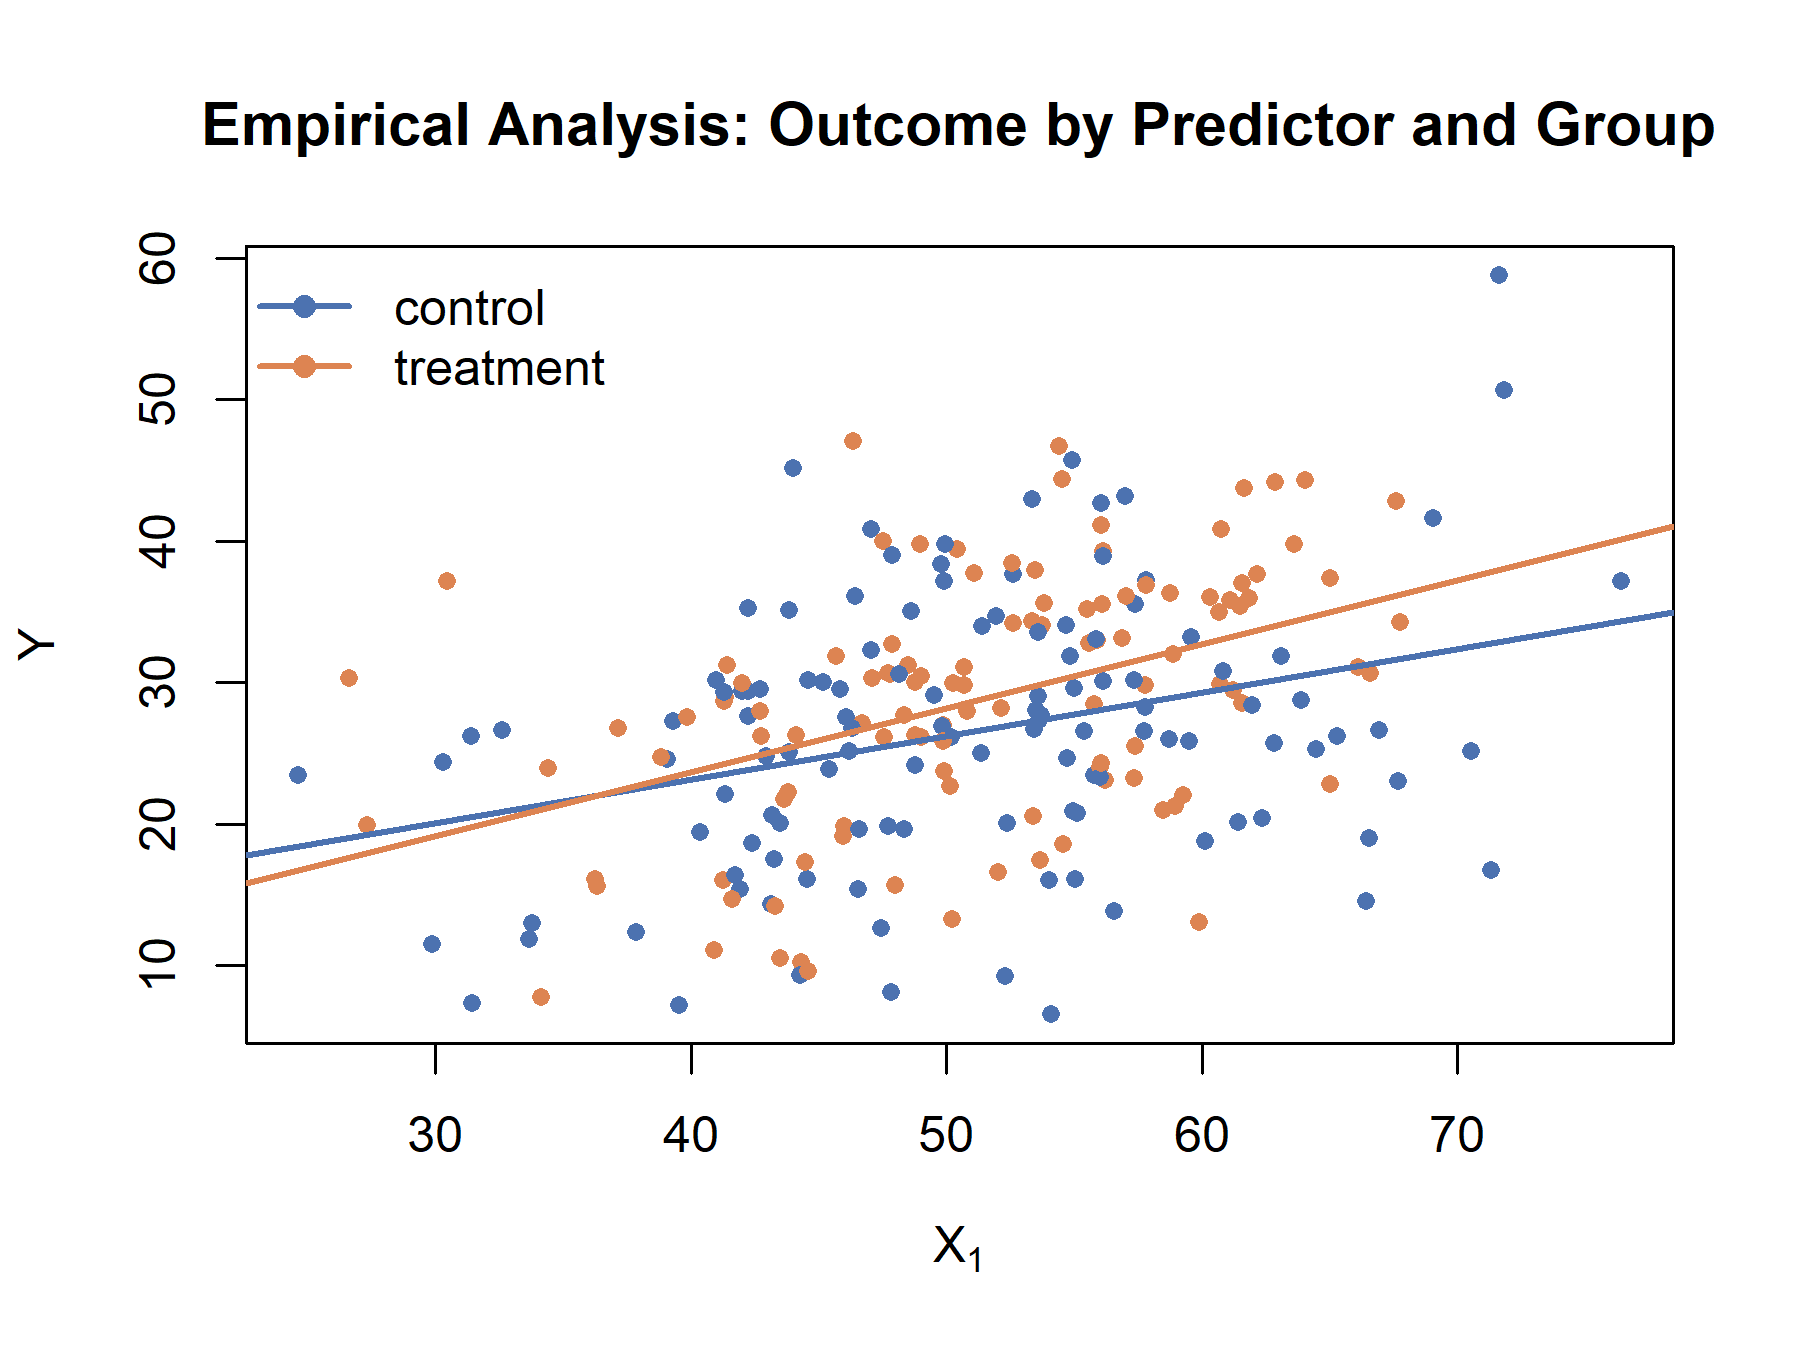
\includegraphics[width=0.7\textwidth]{empirical/figures/fig_empirical.png}
  \figurenote{Points are individual observations; lines are group-wise fitted values.}
\end{figure}

\section{Discussion}

What were your main aims? What were key findings regarding each aim?

Compare and contrast findings observed to past literature.
\subsection{Limitations and Future Directions}

At least 2 limitations. How do your findings contribute to existing literature? 

How should we move forward in research or practice given your contribution to the literature?

\subsection{Conclusion}

Summarize the key takeaways of your paper.


% ---------- References ----------
\printbibliography

% ---------- Appendices ----------
% \appendix
% \section{Supplementary Materials}
% \label{app:supplement}

\end{document}
